\documentclass[11pt,handout]{beamer}
\usepackage[utf8]{inputenc}
\usepackage[T1]{fontenc}
\usepackage{lmodern}
\usepackage[english]{babel}
\usepackage{graphicx}
\usepackage[most]{tcolorbox}
\usetheme{Darmstadt}
\setbeamertemplate{navigation symbols}{}
\setbeamertemplate{footline}{
	\begin{beamercolorbox}[ht=3ex,leftskip=1.4cm,rightskip=.3cm]{author in head/foot}
		\hfill \insertframenumber
		\vspace*{0.07cm}
	\end{beamercolorbox}
} 
\usepackage{url}
\usepackage{hyperref}
\usepackage{listings}

% color def
\usepackage{color}
\definecolor{darkred}{rgb}{0.6,0.0,0.0}
\definecolor{darkgreen}{rgb}{0,0.50,0}
\definecolor{lightblue}{rgb}{0.0,0.42,0.91}
\definecolor{orange}{rgb}{0.99,0.48,0.13}
\definecolor{grass}{rgb}{0.18,0.80,0.18}
\definecolor{pink}{rgb}{0.97,0.15,0.45}

\usepackage{nth}

% General Setting of listings
\lstset{
	language=Python,
	tabsize=4,
	aboveskip=1em,
	breaklines=true,
	abovecaptionskip=-6pt,
	captionpos=b,
	escapeinside={\%*}{*)},
	frame=single,
	numbers=left,
	numbersep=8pt,
	numberstyle=\tiny,
	morekeywords=[1]{,as,assert,nonlocal,with,yield,self,True,False,None,} % Python builtin
	morekeywords=[2]{,__init__,__add__,__mul__,__div__,__sub__,__call__,__getitem__,__setitem__,__eq__,__ne__,__nonzero__,__rmul__,__radd__,__repr__,__str__,__get__,__truediv__,__pow__,__name__,__future__,__all__,}, % magic methods
	morekeywords=[3]{,object,type,isinstance,copy,deepcopy,zip,enumerate,reversed,list,set,len,dict,tuple,range,xrange,append,execfile,real,imag,reduce,str,repr,}, % common functions
	morekeywords=[4]{,Exception,NameError,IndexError,SyntaxError,TypeError,ValueError,OverflowError,ZeroDivisionError,}, % errors
	morekeywords=[5]{,ode,fsolve,sqrt,exp,sin,cos,arctan,arctan2,arccos,pi, array,norm,solve,dot,arange,isscalar,max,sum,flatten,shape,reshape,find,any,all,abs,plot,linspace,legend,quad,polyval,polyfit,hstack,concatenate,vstack,column_stack,empty,zeros,ones,rand,vander,grid,pcolor,eig,eigs,eigvals,svd,qr,tan,det,logspace,roll,min,mean,cumsum,cumprod,diff,vectorize,lstsq,cla,eye,xlabel,ylabel,squeeze,}, % numpy / math
	deletekeywords=[2]{next,set},
	deletekeywords=[3]{next,set},
	basicstyle=\ttfamily\small,
	backgroundcolor=\color{white},
	commentstyle=\color{darkgreen}\slshape,
	keywordstyle=\color{blue}\bfseries\itshape,
	keywordstyle=[2]\color{blue}\bfseries,
	keywordstyle=[3]\color{grass},
	keywordstyle=[4]\color{red},
	keywordstyle=[5]\color{orange},
	stringstyle=\color{darkred},
	emphstyle=\color{pink}\underbar,
	morestring=*[d]{"},
}

\usepackage{tikz}
\usetikzlibrary{calc,shapes.multipart,chains,arrows,positioning,overlay-beamer-styles}
\tikzstyle{vertex}=[draw,fill=white!15,circle,minimum size=20pt,inner sep=1pt]



\begin{document}
	\author{Data Structures}
	\title{Trees}
	\titlegraphic{
\includegraphics[width=3cm]{img/UPNA}}
	\date[]{2024-2025}
	\subject{Data Structures}
	%\subtitle{}
	%\logo{}
	%\institute{}
	%\date{}
	%\subject{}
	%\setbeamercovered{transparent}
	%\setbeamertemplate{navigation symbols}{}
	\begin{frame}[plain]
		\maketitle
	\end{frame}

	\begin{frame}
		\tableofcontents
	\end{frame}

\section{What is a Tree?}

\subsection{Trees in Computer Science}

\begin{frame}\frametitle{Tree Definition}
\begin{itemize}
\item A tree is a subset of a graph
    \begin{itemize}
    \item There are no cycles
    \end{itemize}
\item They have nothing in common with real trees
    \begin{itemize}
    \item Thought they copy a lot of the nomenclature
    \end{itemize}
\end{itemize}
\pause
\begin{block}{}
\centering\Large A hierarchical way to store data
\end{block}
\end{frame}

\begin{frame}\frametitle{Recursive Tree of the Fibonacci Sequence}
\begin{center}
\scalebox{0.9}{
\begin{tikzpicture}[very thick,level/.style={sibling distance=60mm/####1}, level 3/.style={sibling distance=12mm}, level 4/.style={sibling distance=12mm}]
\node [vertex] (r){$fib(5)$}
  child {
    node [vertex] (a) {$fib(4)$}
    child {
      node [vertex] {$fib(3)$}
      child {
        node [vertex] {$fib(2)$}
        child {
            node [vertex] {$fib(1)$}
        }
        child {
            node [vertex] {$fib(0)$}
        }
      }
      child {
        node [vertex] {$fib(1)$}
      }
    }
    child {
      node [vertex] {$fib(2)$}
      child {
          node [vertex] {$fib(1)$}
      }
      child {
          node [vertex] {$fib(0)$}
      }
    }
  }
  child {
    node [vertex] {$fib(3)$}
    child {
      node [vertex] {$fib(2)$}
      child {
            node [vertex] {$fib(1)$}
        }
        child {
            node [vertex] {$fib(0)$}
        }
    }
    child {
      node [vertex] {$fib(1)$}
    }
  };
\end{tikzpicture}
}
\end{center}
\end{frame}


\tikzstyle{vertex}=[draw,fill=white!15,circle,minimum size=1.4cm,inner sep=1pt]
\begin{frame}\frametitle{Tree Parts}
\begin{center}
\scalebox{0.9}{
\begin{tikzpicture}[very thick,level/.style={sibling distance=40mm/####1}, level distance=20mm,every edge/.style = {draw, -latex, thick}]
\node [vertex] (r){root}
    child {
        node [vertex] {branch}
        child {
            node [vertex] {leaf}
        }
    }
    child {
        node [vertex] {branch}
        child {
            node [vertex] {leaf}
        }
        child {
            node [vertex] {leaf}
        }
    }
    child {
        node [vertex] (b) {branch}
        child {
            node [vertex] {branch}
            child {
                node [vertex] {leaf}
            }
        }
    };
\end{tikzpicture}
}
\end{center}
\end{frame}

\begin{frame}\frametitle{Vertex Relationship}
\begin{center}
\scalebox{0.9}{
\begin{tikzpicture}[very thick,level/.style={sibling distance=40mm/####1}, level distance=20mm,every edge/.style = {draw, -latex, thick}]
\node [vertex] (r){root}
    child {
        node [vertex] {branch}
        child {
            node [vertex] {leaf}
        }
    }
    child {
        node [vertex] {branch}
        child {
            node [vertex] {leaf}
        }
        child {
            node [vertex] {leaf}
        }
    }
    child {
        node [vertex] (b) {branch}
        child {
            node [vertex] {branch}
            child {
                node [vertex] {leaf}
            }
        }
    };
    
\draw[green] (b.north) edge[out=90, in=0] node[above]{parent} (r.east) ;
\draw[green] (r.south east) edge[out=-45, in=180] node[below=0.4cm]{child} (b.west) ;
\end{tikzpicture}
}
\end{center}
\end{frame}

\begin{frame}\frametitle{Characteristics}
\begin{itemize}
\item Each branch of a tree creates a \textbf{subtree}
    \begin{itemize}
    \item We can treat this as a smaller tree
    \item The tree structure is recursively defined
    \end{itemize}
\item We can define two characteristics for any tree:
\begin{description}
\item[Height:] Maximum number of levels the tree has
\item[Weight:] Number of nodes the tree has
\end{description}
\end{itemize}
\end{frame}


\begin{frame}\frametitle{Characteristics II}
\begin{center}
\begin{block}{}
\centering\Large What is this tree's height?
\end{block}
\vspace{0.5cm}
\scalebox{0.7}{
\begin{tikzpicture}[very thick,level/.style={sibling distance=40mm/####1}, level distance=20mm,every edge/.style = {draw, -latex, thick}]
\node [vertex] (r){root}
    child {
        node [vertex] {branch}
        child {
            node [vertex] {leaf}
        }
    }
    child {
        node [vertex] {branch}
        child {
            node [vertex] {leaf}
        }
        child {
            node [vertex] {leaf}
        }
    }
    child {
        node [vertex] (b) {branch}
        child {
            node [vertex] {branch}
            child {
                node [vertex] {leaf}
            }
        }
    };
\end{tikzpicture}
}
\end{center}
\end{frame}

\begin{frame}\frametitle{Characteristics III}
\begin{center}
\begin{block}{}
\centering\Large And its weight?
\end{block}
\vspace{0.5cm}
\scalebox{0.7}{
\begin{tikzpicture}[very thick,level/.style={sibling distance=40mm/####1}, level distance=20mm,every edge/.style = {draw, -latex, thick}]
\node [vertex] (r){root}
    child {
        node [vertex] {branch}
        child {
            node [vertex] {leaf}
        }
    }
    child {
        node [vertex] {branch}
        child {
            node [vertex] {leaf}
        }
        child {
            node [vertex] {leaf}
        }
    }
    child {
        node [vertex] (b) {branch}
        child {
            node [vertex] {branch}
            child {
                node [vertex] {leaf}
            }
        }
    };
\end{tikzpicture}
}
\end{center}
\end{frame}

\section{Binary Trees}

\subsection{What is a Binary Tree}

\begin{frame}\frametitle{Limiting a Tree}
\begin{itemize}
\item As with any structure, we can add specifications on how we use a tree
\item One common restriction is to limit each node to \textbf{two children}
    \begin{itemize}
    \item Due to the recursive nature of the trees, this means that each node has two subtrees
    \item We can name each child as \textbf{left} or \textbf{right}
    \end{itemize}
\end{itemize}
\pause
\begin{block}{}
\centering\Large Binary Tree
\end{block}
\end{frame}

\begin{frame}\frametitle{Binary Tree Nomenclature I}
\begin{block}{}
\centering\Large Full node \vphantom{\Large Empty node}
\end{block}
\vspace{0.5cm}
\begin{center}
\scalebox{0.6}{
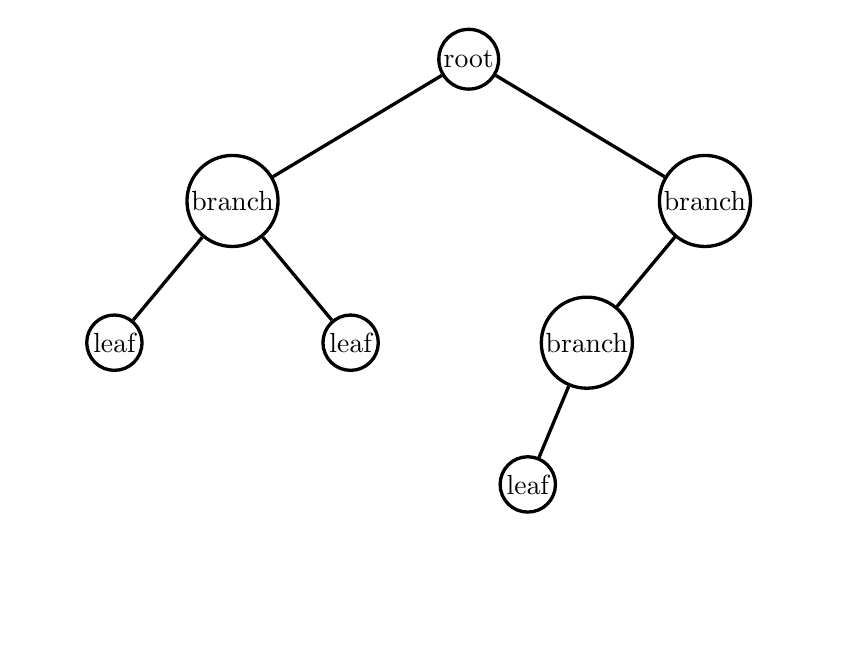
\begin{tikzpicture}[very thick,
level 1/.style={sibling distance=60mm}, 
level 2/.style={sibling distance=30mm}, 
level 3/.style={sibling distance=15mm}, 
level 4/.style={sibling distance=15mm}, 
level distance=18mm,every edge/.style = {draw, -latex, thick}]
\node [vertex, alt=<2>{fill=blue!30}{fill=white}] (r){root}
    child {
        node [vertex, alt=<2>{fill=blue!30}{fill=white}] {branch}
        child {
            node [vertex] {leaf}
            child {
                node[vertex,draw=none] {} edge from parent[draw=none] 
            }
            child {
                node[draw=none] {} edge from parent[draw=none] 
            }
        }
        child {
            node [vertex] {leaf}
        }
    }
    child {
        node [vertex] (b) {branch}
        child {
            node [vertex] {branch}
            child {
                node [vertex] {leaf}
                child {
                    node[draw=none] {} edge from parent[draw=none]  
                }
                child {
                    node[draw=none] {} edge from parent[draw=none]   
                }
            }
            child {
                node[draw=none] {} edge from parent[draw=none]   
            }
        }
        child {
            node[draw=none] {} edge from parent[draw=none]  
        }
    };
\end{tikzpicture}
}
\end{center}
\end{frame}

\begin{frame}\frametitle{Binary Tree Nomenclature II}
\begin{block}{}
\centering\Large Empty node \vphantom{\Large Full node}
\end{block}
\vspace{0.5cm}
\begin{center}
\scalebox{0.6}{
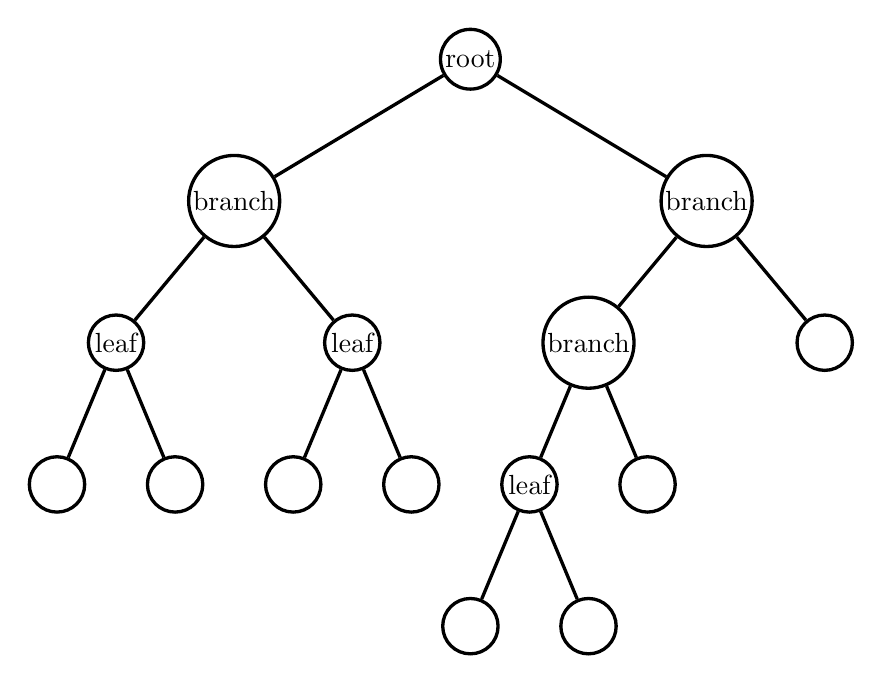
\begin{tikzpicture}[very thick,
level 1/.style={sibling distance=60mm}, 
level 2/.style={sibling distance=30mm}, 
level 3/.style={sibling distance=15mm}, 
level 4/.style={sibling distance=15mm}, 
level distance=18mm,every edge/.style = {draw, -latex, thick}]
\node [vertex] (r){root}
    child {
        node [vertex] {branch}
        child {
            node [vertex] {leaf}
            child {
                node[vertex,alt=<2>{draw=black,dotted}{draw=none}] {} edge from parent[alt=<2>{draw=black,dotted}{draw=none}] 
            }
            child {
                node[vertex,alt=<2>{draw=black,dotted}{draw=none}] {} edge from parent[alt=<2>{draw=black,dotted}{draw=none}] 
            }
        }
        child {
            node [vertex] {leaf}
            child {
                node[vertex,alt=<2>{draw=black,dotted}{draw=none}] {} edge from parent[alt=<2>{draw=black,dotted}{draw=none}] 
            }
            child {
                node[vertex,alt=<2>{draw=black,dotted}{draw=none}] {} edge from parent[alt=<2>{draw=black,dotted}{draw=none}] 
            }
        }
    }
    child {
        node [vertex] (b) {branch}
        child {
            node [vertex] {branch}
            child {
                node [vertex] {leaf}
                child {
                    node[vertex,alt=<2>{draw=black,dotted}{draw=none}] {} edge from parent[alt=<2>{draw=black,dotted}{draw=none}]  
                }
                child {
                    node[vertex,alt=<2>{draw=black,dotted}{draw=none}] {} edge from parent[alt=<2>{draw=black,dotted}{draw=none}]  
                }
            }
            child {
                node[vertex,alt=<2>{draw=black,dotted}{draw=none}] {} edge from parent[alt=<2>{draw=black,dotted}{draw=none}]  
            }
        }
        child {
            node[vertex,alt=<2>{draw=black,dotted}{draw=none}] {} edge from parent[alt=<2>{draw=black,dotted}{draw=none}] 
        }
    };
\end{tikzpicture}
}
\end{center}
\end{frame}

\begin{frame}\frametitle{Binary Tree Nomenclature III}
\begin{block}{}
\centering\Large Full Binary Tree \vphantom{\Large Empty node}
\end{block}
\vspace{0.5cm}
\begin{center}
\scalebox{0.6}{
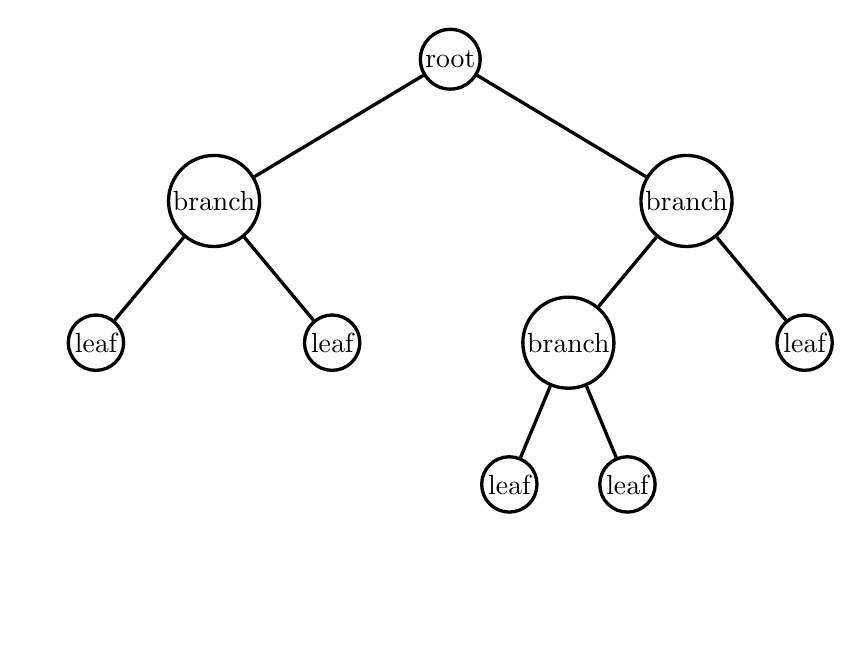
\begin{tikzpicture}[very thick,
level 1/.style={sibling distance=60mm}, 
level 2/.style={sibling distance=30mm}, 
level 3/.style={sibling distance=15mm}, 
level 4/.style={sibling distance=15mm}, 
level distance=18mm,every edge/.style = {draw, -latex, thick}]
\node [vertex] (r){root}
    child {
        node [vertex] {branch}
        child {
            node [vertex] {leaf}
            child {
                node[draw=none] {} edge from parent[draw=none]  
            }
            child {
                node[draw=none] {} edge from parent[draw=none]  
            }
        }
        child {
            node [vertex] {leaf}
        }
    }
    child {
        node [vertex] (b) {branch}
        child {
            node [vertex] {branch}
            child {
                node [vertex] {leaf}
                child {
                    node[draw=none] {} edge from parent[draw=none]   
                }
                child {
                    node[draw=none] {} edge from parent[draw=none]   
                }
            }
            child {
                node [vertex] {leaf}  
            }
        }
        child {
            node [vertex] {leaf}
        }
    };
\end{tikzpicture}
}
\end{center}
\end{frame}

\begin{frame}\frametitle{Symmetric Trees}
\begin{block}{}
\centering Trees where the left and right subtrees have the \textbf{same structure} (but inverted) with the \textbf{same values} for all nodes
\end{block}
\vspace{0.5cm}
\begin{center}
\scalebox{0.6}{
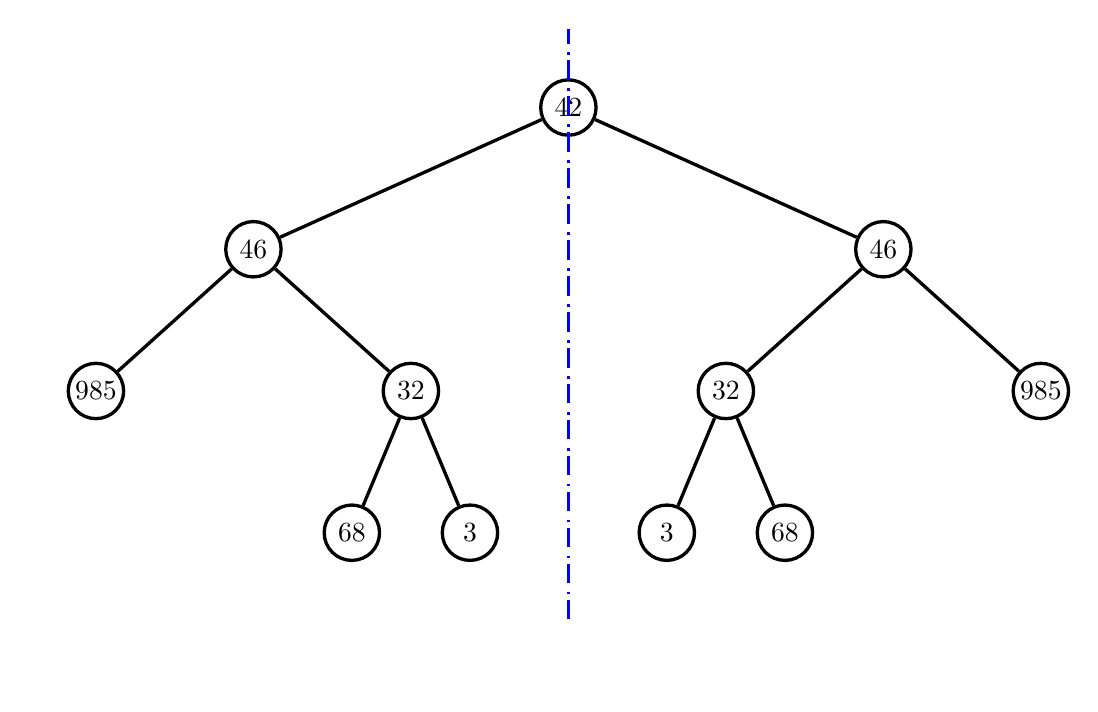
\begin{tikzpicture}[very thick,
level 1/.style={sibling distance=80mm}, 
level 2/.style={sibling distance=40mm}, 
level 3/.style={sibling distance=15mm}, 
level 4/.style={sibling distance=15mm}, 
level distance=18mm,every edge/.style = {draw, -latex, thick}]
\node [vertex] (r){42}
    child {
        node [vertex] {46}
        child {
            node [vertex] {985}
            child {
                node[draw=none] {} edge from parent[draw=none]  
            }
            child {
                node[draw=none] {} edge from parent[draw=none]  
            }
        }
        child {
            node [vertex] {32}
            child {
                node [vertex] {68}
                child {
                    node[draw=none] {} edge from parent[draw=none]   
                }
                child {
                    node[draw=none] {} edge from parent[draw=none]   
                }
            }
            child {
                node [vertex] {3}  
            }
        }
    }
    child {
        node [vertex] (b) {46}
        child {
            node [vertex] {32}
            child {
                node [vertex] {3}
                child {
                    node[draw=none] {} edge from parent[draw=none]   
                }
                child {
                    node[draw=none] {} edge from parent[draw=none]   
                }
            }
            child {
                node [vertex] {68}  
            }
        }
        child {
            node [vertex] {985}
        }
    };
\draw [thick,dash pattern={on 7pt off 2pt on 1pt off 3pt}, blue] (0,-6.5) -- (0,1);
\end{tikzpicture}
}
\end{center}
\end{frame}

\subsection{Tree Traversal}

\begin{frame}\frametitle{How to Visit Nodes}
\begin{description}
\item[Pre-order:] First the node value, then the left subtree and finally the right subtree
\item[In-order:] First the left subtree, then the node value, and finally the right subtree
\item[Post-order:] First the left subtree, then the right subtree and finally the node value
\end{description}
\end{frame}


\begin{frame}\frametitle{Pre-order}
\begin{block}{}
\centering First the node value, then the left subtree and finally the right subtree
\end{block}
\begin{center}
\scalebox{0.6}{
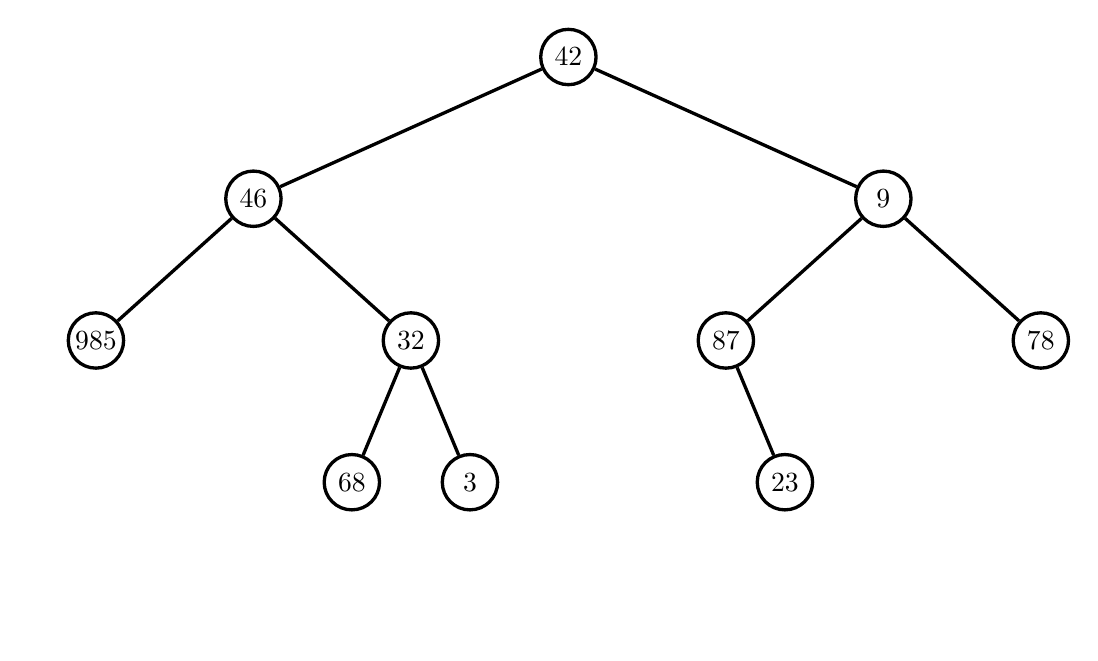
\begin{tikzpicture}[very thick,
level 1/.style={sibling distance=80mm}, 
level 2/.style={sibling distance=40mm}, 
level 3/.style={sibling distance=15mm}, 
level 4/.style={sibling distance=15mm}, 
level distance=18mm,every edge/.style = {draw, -latex, thick}]
\node [vertex] (r){42}
    child {
        node [vertex] {46}
        child {
            node [vertex] {985}
            child {
                node[draw=none] {} edge from parent[draw=none]  
            }
            child {
                node[draw=none] {} edge from parent[draw=none]  
            }
        }
        child {
            node [vertex] {32}
            child {
                node [vertex] {68}
                child {
                    node[draw=none] {} edge from parent[draw=none]   
                }
                child {
                    node[draw=none] {} edge from parent[draw=none]   
                }
            }
            child {
                node [vertex] {3}  
            }
        }
    }
    child {
        node [vertex] (b) {9}
        child {
            node [vertex] {87}
            child {
                node[draw=none] {} edge from parent[draw=none]   
                child {
                    node[draw=none] {} edge from parent[draw=none]   
                }
                child {
                    node[draw=none] {} edge from parent[draw=none]   
                }
            }
            child {
                node [vertex] {23}  
            }
        }
        child {
            node [vertex] {78}
        }
    };
\end{tikzpicture}
}
\end{center}
\end{frame}

\begin{frame}\frametitle{In-order}
\begin{block}{}
\centering First the left subtree, then the node value, and finally the right subtree
\end{block}
\begin{center}
\scalebox{0.6}{
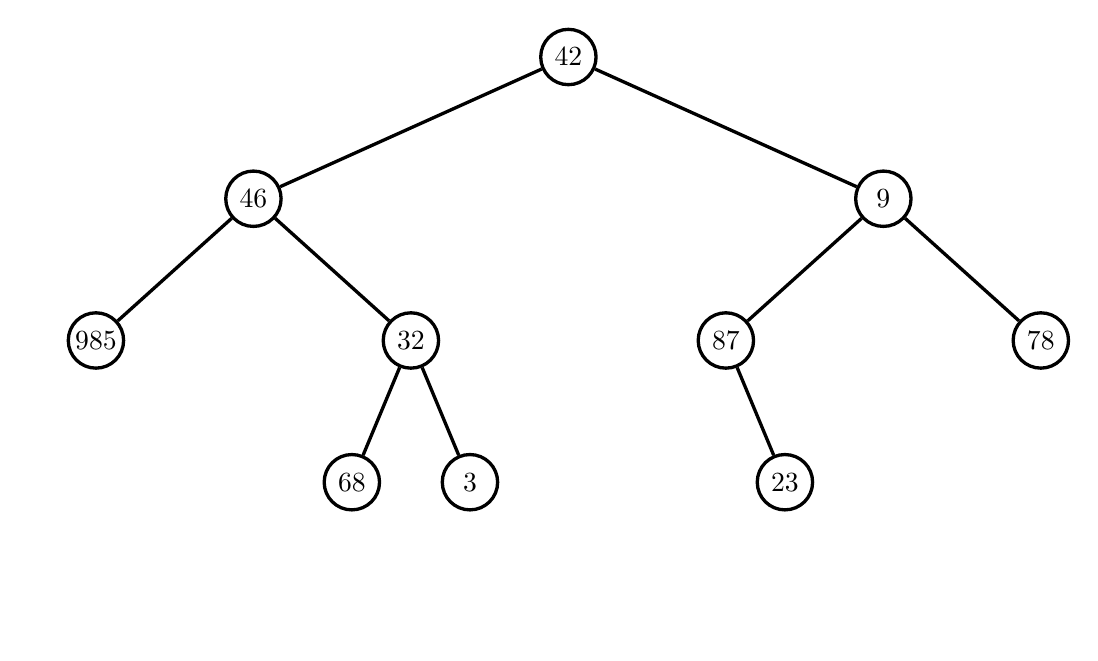
\begin{tikzpicture}[very thick,
level 1/.style={sibling distance=80mm}, 
level 2/.style={sibling distance=40mm}, 
level 3/.style={sibling distance=15mm}, 
level 4/.style={sibling distance=15mm}, 
level distance=18mm,every edge/.style = {draw, -latex, thick}]
\node [vertex] (r){42}
    child {
        node [vertex] {46}
        child {
            node [vertex] {985}
            child {
                node[draw=none] {} edge from parent[draw=none]  
            }
            child {
                node[draw=none] {} edge from parent[draw=none]  
            }
        }
        child {
            node [vertex] {32}
            child {
                node [vertex] {68}
                child {
                    node[draw=none] {} edge from parent[draw=none]   
                }
                child {
                    node[draw=none] {} edge from parent[draw=none]   
                }
            }
            child {
                node [vertex] {3}  
            }
        }
    }
    child {
        node [vertex] (b) {9}
        child {
            node [vertex] {87}
            child {
                node[draw=none] {} edge from parent[draw=none]   
                child {
                    node[draw=none] {} edge from parent[draw=none]   
                }
                child {
                    node[draw=none] {} edge from parent[draw=none]   
                }
            }
            child {
                node [vertex] {23}  
            }
        }
        child {
            node [vertex] {78}
        }
    };
\end{tikzpicture}
}
\end{center}
\end{frame}

\begin{frame}\frametitle{Post-order}
\begin{block}{}
\centering First the left subtree, then the right subtree and finally the node value
\end{block}
\begin{center}
\scalebox{0.6}{
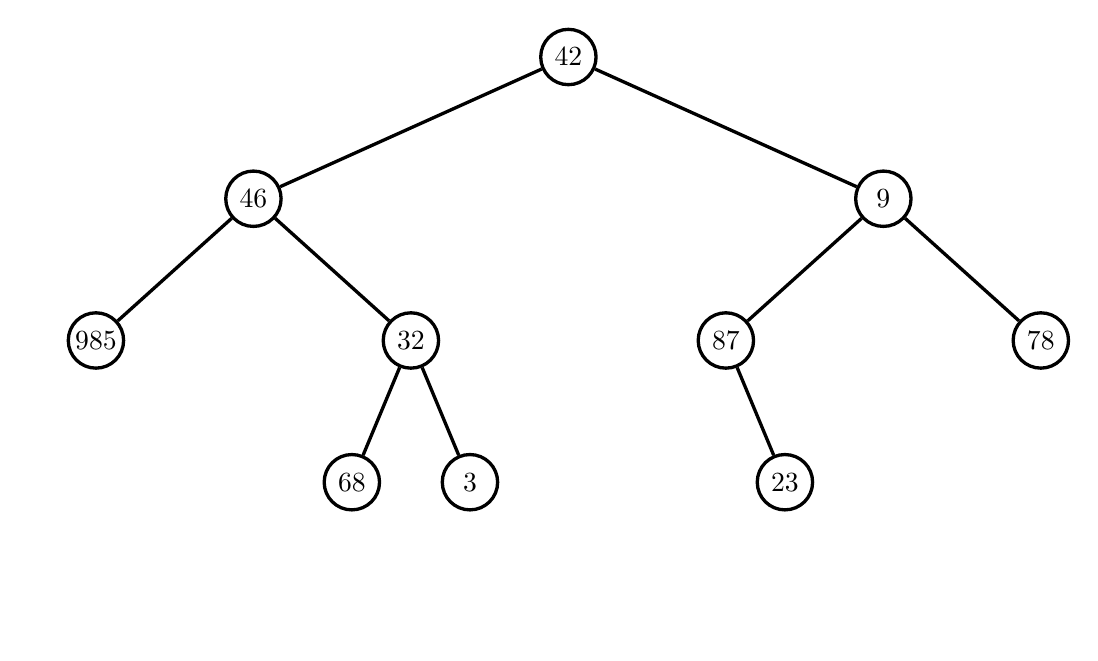
\begin{tikzpicture}[very thick,
level 1/.style={sibling distance=80mm}, 
level 2/.style={sibling distance=40mm}, 
level 3/.style={sibling distance=15mm}, 
level 4/.style={sibling distance=15mm}, 
level distance=18mm,every edge/.style = {draw, -latex, thick}]
\node [vertex] (r){42}
    child {
        node [vertex] {46}
        child {
            node [vertex] {985}
            child {
                node[draw=none] {} edge from parent[draw=none]  
            }
            child {
                node[draw=none] {} edge from parent[draw=none]  
            }
        }
        child {
            node [vertex] {32}
            child {
                node [vertex] {68}
                child {
                    node[draw=none] {} edge from parent[draw=none]   
                }
                child {
                    node[draw=none] {} edge from parent[draw=none]   
                }
            }
            child {
                node [vertex] {3}  
            }
        }
    }
    child {
        node [vertex] (b) {9}
        child {
            node [vertex] {87}
            child {
                node[draw=none] {} edge from parent[draw=none]   
                child {
                    node[draw=none] {} edge from parent[draw=none]   
                }
                child {
                    node[draw=none] {} edge from parent[draw=none]   
                }
            }
            child {
                node [vertex] {23}  
            }
        }
        child {
            node [vertex] {78}
        }
    };
\end{tikzpicture}
}
\end{center}
\end{frame}

\subsection{Creating a Tree on Python}

\begin{frame}[fragile]\frametitle{Creating a Tree}
\begin{itemize}
\item We can create a tree by using a simple list
\end{itemize}
\begin{lstlisting}
left = [...]
right = [...]
node = [value, left, right]
\end{lstlisting}
\pause
\begin{alertblock}{}
\centering \Large We will leave this for crazy people
\end{alertblock}
\end{frame}

\begin{frame}[fragile]\frametitle{Creating a Tree II}
\begin{itemize}
\item Using Python we can use classes to define our node
\end{itemize}
\pause
\begin{lstlisting}
class BinaryTreeNode:
    def __init__(self, value):
        self.value = value
        self.left =  None
        self.right = None
\end{lstlisting}
\end{frame}

\subsection{Exercises}

\begin{frame}\frametitle{Exercises}
\begin{block}{Exercise I}
Create a method called \lstinline|insert_left(node, value)|, that takes a \lstinline|BinaryTreeNode| and a value, and tries to insert it on the left subtree of that node. Do the same for \lstinline|insert_right|.
\end{block}
\begin{center}
\scalebox{0.8}{
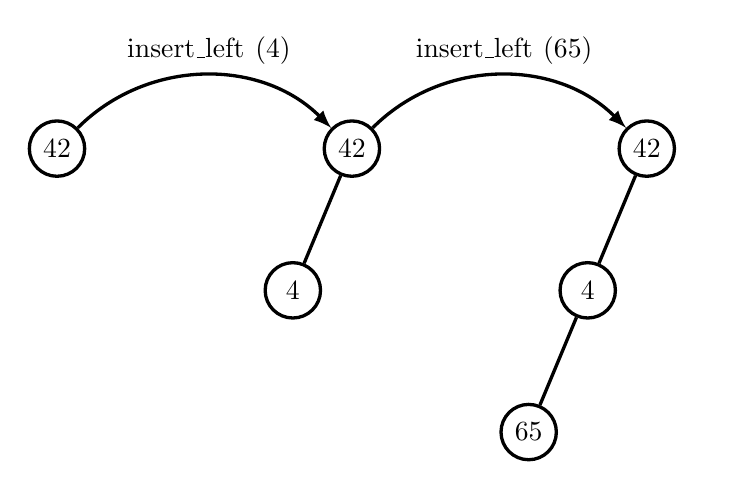
\begin{tikzpicture}[very thick,
level 1/.style={sibling distance=15mm}, 
level 2/.style={sibling distance=15mm}, 
level 3/.style={sibling distance=15mm}, 
level 4/.style={sibling distance=15mm}, 
level distance=18mm,every edge/.style = {draw, -latex, thick}]
\node[vertex] (a) {42};

\node[vertex, right=3cm of a] (b) {42}
    child {
        node[vertex] {4}
    }
    child{
        node[draw=none] {} edge from parent[draw=none] 
    };
    
\node[vertex, right=3cm of b] (c) {42}
    child {
        node[vertex] {4}
        child {
            node[vertex] {65}
        }
        child{
            node[draw=none] {} edge from parent[draw=none] 
        }
    }
    child{
        node[draw=none] {} edge from parent[draw=none] 
    };
    
\draw[-{latex}] (a) to[out=45, in=135] node[midway, above] {\lstinline|insert_left(4)|} (b);
\draw[-{latex}] (b) to[out=45, in=135] node[midway, above] {\lstinline|insert_left(65)|} (c);
\end{tikzpicture}
}
\end{center}
\end{frame}

\begin{frame}\frametitle{Exercises}
\begin{block}{Exercise II}
Having functions hanging around the code might make the structure more complex. Why not centralize everything in a single class, as with the \lstinline|LinkedList|?

Use the class \lstinline|BinnaryTreeNode| and add the functions as methods of the class.
\end{block}
\end{frame}

\begin{frame}\frametitle{Exercises}
\begin{block}{Exercise III}
Create a method that calculates the number of levels or \textbf{height} of a given tree. Call it \lstinline|get_heigth(self)|.

Tip: you can delegate the calculation to the subtrees, until you reach the end. Then choose the maximum of both branches and add one.
\end{block}
\begin{block}{Exercise IV}
Create a method that calculates the size or \textbf{weight} of a given tree. Call it \lstinline|get_weight(self)|.

Tip: you can again ask the branches for their weight.
\end{block}
\end{frame}

\begin{frame}\frametitle{Exercises}
\begin{block}{Exercise V}
Create a method, \lstinline|print_pre_order(self)|, that will print the tree following pre-ordering. Remember first the node value, then the left subtree and finally the right subtree.
\end{block}
\begin{block}{Exercise VI}
Create a method, \lstinline|print_in_order(self)|, that will print the tree following in-ordering. Remember first the left subtree, then the node value, and finally the right subtree.
\end{block}
\begin{block}{Exercise VII}
Create a method, \lstinline|print_post_order(self)|, that will print the tree following post-ordering. Remember first the left subtree, then the right subtree and finally the node value.
\end{block}
\end{frame}

\begin{frame}\frametitle{Completing the BinaryTreeNode}
\begin{itemize}
\item How can we delete a node?
    \begin{itemize}
    \item Does deleting any node have the same complexity?
    \end{itemize}
\item Can we check if the tree contains a value?
\item Can we change the insertion criteria?
    \begin{itemize}
    \item Insert into the branch with the lowest weight?
    \item Insert into the branch with the lowest height?
    \item What would happen if we only insert on the left?
    \end{itemize}
\item What is a balanced tree?
    \begin{itemize}
    \item How can we keep it balanced?
    \end{itemize}
\end{itemize}
\end{frame}

\subsection{Binary Search Trees}


\begin{frame}\frametitle{A Binary Search Tree}
\begin{block}{}
\centering Do you see anything different on this tree?
\end{block}
\begin{center}
\scalebox{0.6}{
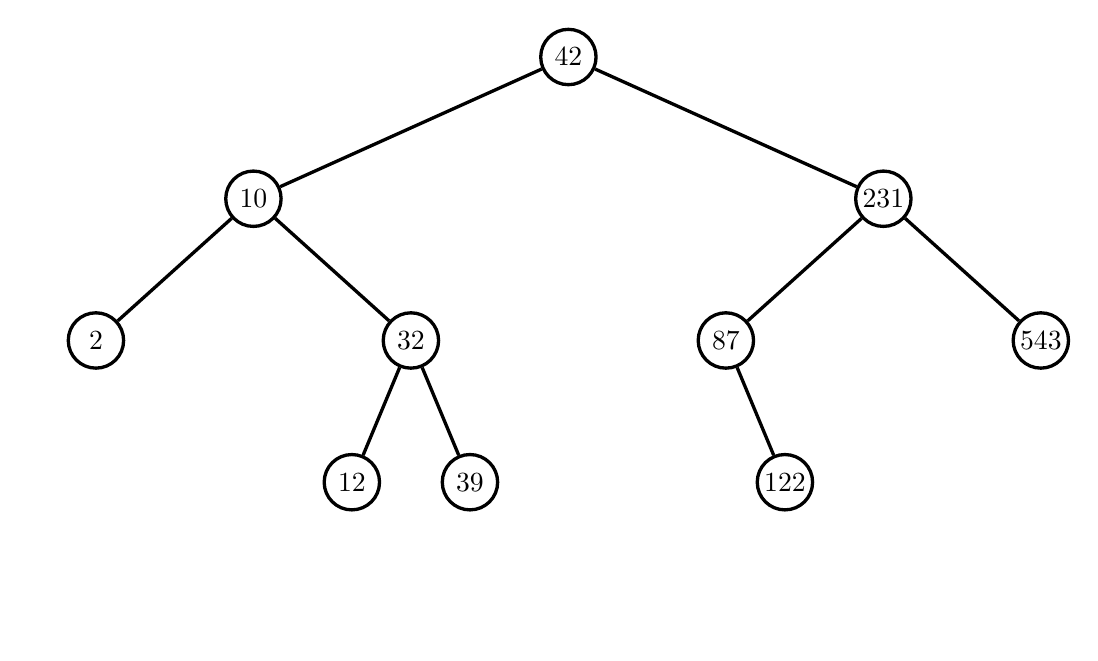
\begin{tikzpicture}[very thick,
level 1/.style={sibling distance=80mm}, 
level 2/.style={sibling distance=40mm}, 
level 3/.style={sibling distance=15mm}, 
level 4/.style={sibling distance=15mm}, 
level distance=18mm,every edge/.style = {draw, -latex, thick}]
\node [vertex] (r){42}
    child {
        node [vertex] {10}
        child {
            node [vertex] {2}
            child {
                node[draw=none] {} edge from parent[draw=none]  
            }
            child {
                node[draw=none] {} edge from parent[draw=none]  
            }
        }
        child {
            node [vertex] {32}
            child {
                node [vertex] {12}
                child {
                    node[draw=none] {} edge from parent[draw=none]   
                }
                child {
                    node[draw=none] {} edge from parent[draw=none]   
                }
            }
            child {
                node [vertex] {39}  
            }
        }
    }
    child {
        node [vertex] (b) {231}
        child {
            node [vertex] {87}
            child {
                node[draw=none] {} edge from parent[draw=none]   
                child {
                    node[draw=none] {} edge from parent[draw=none]   
                }
                child {
                    node[draw=none] {} edge from parent[draw=none]   
                }
            }
            child {
                node [vertex] {122}  
            }
        }
        child {
            node [vertex] {543}
        }
    };
\end{tikzpicture}
}
\end{center}
\end{frame}

\begin{frame}\frametitle{Limiting Insertion}
\begin{itemize}
\item We can further limit how we handle insertion by choosing a position based on the value to insert
\item A Binary Search Tree only adds a small restriction
    \begin{itemize}
    \item The left subtree contains values that are smaller
    \item The right subtree contains values that are bigger
    \end{itemize}
\item We will not be able to specify where to insert
    \begin{itemize}
    \item The tree will choose a position
    \item Recursively insert left or right
    \end{itemize}
\item The main benefit we obtain is that we have fast access to data
    \begin{itemize}
    \item We only have to look at a fraction of the tree
    \end{itemize}
\end{itemize}
\end{frame}

\begin{frame}\frametitle{A Small Change Creates Huge Complications}
\begin{itemize}
\item How can we delete a node?
\begin{description}
\item[Node is leaf:] Simply delete it
\item[Node has 1 child:] Child becomes the node
\item[Node has 2 children:] Find the in-order successor (the predecessor can also be used), swap places, and then delete the node.
\end{description}
\end{itemize}
\end{frame}

\end{document}






